\documentclass{article}

% Hier befinden sich Pakete, die wir beinahe immer benutzen ...

\usepackage[utf8]{inputenc}

% Sprach-Paket:
\usepackage[ngerman]{babel}

% damit's nicht so, wie beim Grill aussieht:
\usepackage{fullpage}

% Mathematik:
\usepackage{amsmath, amssymb, amsfonts, amsthm}
\usepackage{bbm}
\usepackage{mathtools, mathdots}

% Makros mit mehereren Default-Argumenten:
\usepackage{twoopt}

% Anführungszeichen (Makro \Quote{}):
\usepackage{babel}

% if's für Makros:
\usepackage{xifthen}
\usepackage{etoolbox}

% tikz ist kein Zeichenprogramm (doch!):
\usepackage{tikz}

% bessere Aufzählungen:
\usepackage{enumitem}

% (bessere) Umgebung für Bilder:
\usepackage{graphicx, subfig, float}

% Umgebung für Code:
\usepackage{listings}

% Farben:
\usepackage{xcolor}

% Umgebung für "plain text":
\usepackage{verbatim}

% Umgebung für mehrerer Spalten:
\usepackage{multicol}

% "nette" Brüche
\usepackage{nicefrac}

% Spaltentypen verschiedener Dicke
\usepackage{tabularx}
\usepackage{makecell}

% Für Vektoren
\usepackage{esvect}

% (Web-)Links
\usepackage{hyperref}

% Zitieren & Literatur-Verzeichnis
\usepackage[style = authoryear]{biblatex}
\usepackage{csquotes}

% so ähnlich wie mathbb
%\usepackage{mathds}

% Keine Ahnung, was das macht ...
\usepackage{booktabs}
\usepackage{ngerman}
\usepackage{placeins}

% special letters:

\newcommand{\N}{\mathbb{N}}
\newcommand{\Z}{\mathbb{Z}}
\newcommand{\Q}{\mathbb{Q}}
\newcommand{\R}{\mathbb{R}}
\newcommand{\C}{\mathbb{C}}
\newcommand{\K}{\mathbb{K}}
\newcommand{\T}{\mathbb{T}}
\newcommand{\E}{\mathbb{E}}
\newcommand{\V}{\mathbb{V}}
\renewcommand{\S}{\mathbb{S}}
\renewcommand{\P}{\mathbb{P}}
\newcommand{\1}{\mathbbm{1}}

% quantors:

\newcommand{\Forall}{\forall \,}
\newcommand{\Exists}{\exists \,}
\newcommand{\ExistsOnlyOne}{\exists! \,}
\newcommand{\nExists}{\nexists \,}
\newcommand{\ForAlmostAll}{\forall^\infty \,}

% MISC symbols:

\newcommand{\landau}{{\scriptstyle \mathcal{O}}}
\newcommand{\Landau}{\mathcal{O}}


\newcommand{\eps}{\mathrm{eps}}

% graphics in a box:

\newcommandtwoopt
{\includegraphicsboxed}[3][][]
{
  \begin{figure}[!h]
    \begin{boxedin}
      \ifthenelse{\isempty{#1}}
      {
        \begin{center}
          \includegraphics[width = 0.75 \textwidth]{#3}
          \label{fig:#2}
        \end{center}
      }{
        \begin{center}
          \includegraphics[width = 0.75 \textwidth]{#3}
          \caption{#1}
          \label{fig:#2}
        \end{center}
      }
    \end{boxedin}
  \end{figure}
}

% braces:

\newcommand{\pbraces}[1]{{\left  ( #1 \right  )}}
\newcommand{\bbraces}[1]{{\left  [ #1 \right  ]}}
\newcommand{\Bbraces}[1]{{\left \{ #1 \right \}}}
\newcommand{\vbraces}[1]{{\left  | #1 \right  |}}
\newcommand{\Vbraces}[1]{{\left \| #1 \right \|}}
\newcommand{\abraces}[1]{{\left \langle #1 \right \rangle}}
\newcommand{\round}[1]{\bbraces{#1}}

\newcommand
{\floorbraces}[1]
{{\left \lfloor #1 \right \rfloor}}

\newcommand
{\ceilbraces} [1]
{{\left \lceil  #1 \right \rceil }}

% special functions:

\newcommand{\norm}  [2][]{\Vbraces{#2}_{#1}}
\newcommand{\diam}  [2][]{\mathrm{diam}_{#1} \: #2}
\newcommand{\diag}  [1]{\mathrm{diag} \: #1}
\newcommand{\dist}  [1]{\mathrm{dist} \: #1}
\newcommand{\mean}  [1]{\mathrm{mean} \: #1}
\newcommand{\erf}   [1]{\mathrm{erf} \: #1}
\newcommand{\id}    [1]{\mathrm{id} \: #1}
\newcommand{\sgn}   [1]{\mathrm{sgn} \: #1}
\newcommand{\supp}  [1]{\mathrm{supp} \: #1}
\newcommand{\arsinh}[1]{\mathrm{arsinh} \: #1}
\newcommand{\arcosh}[1]{\mathrm{arcosh} \: #1}
\newcommand{\artanh}[1]{\mathrm{artanh} \: #1}
\newcommand{\card}  [1]{\mathrm{card} \: #1}
\newcommand{\Span}  [1]{\mathrm{span} \: #1}
\newcommand{\Aut}   [1]{\mathrm{Aut} \: #1}
\newcommand{\End}   [1]{\mathrm{End} \: #1}
\newcommand{\ggT}   [1]{\mathrm{ggT} \: #1}
\newcommand{\kgV}   [1]{\mathrm{kgV} \: #1}
\newcommand{\ord}   [1]{\mathrm{ord} \: #1}
\newcommand{\grad}  [1]{\mathrm{grad} \: #1}
\newcommand{\ran}   [1]{\mathrm{ran} \: #1}
\newcommand{\graph} [1]{\mathrm{graph} \: #1}
\newcommand{\Inv}   [1]{\mathrm{Inv} \: #1}
\newcommand{\pv}    [1]{\mathrm{pv} \: #1}
\newcommand{\GL}    [1]{\mathrm{GL} \: #1}
\newcommand{\Mod}{\mathrm{Mod} \:}
\newcommand{\Th}{\mathrm{Th} \:}
\newcommand{\Char}{\mathrm{char}}
\newcommand{\At}{\mathrm{At}}
\newcommand{\Ob}{\mathrm{Ob}}
\newcommand{\Hom}{\mathrm{Hom}}
\newcommand{\orthogonal}[3][]{#2 ~\bot_{#1}~ #3}
\newcommand{\Rang}{\mathrm{Rang}}
\newcommand{\NIL}{\mathrm{NIL}}
\newcommand{\Res}{\mathrm{Res}}
\newcommand{\lxor}{\dot \lor}
\newcommand{\Div}{\mathrm{div} \:}
\newcommand{\meas}{\mathrm{meas} \:}

% fractions:

\newcommand{\Frac}[2]{\frac{1}{#1} \pbraces{#2}}
\newcommand{\nfrac}[2]{\nicefrac{#1}{#2}}

% derivatives & integrals:

\newcommandtwoopt
{\Int}[4][][]
{\int_{#1}^{#2} #3 ~\mathrm{d} #4}

\newcommandtwoopt
{\derivative}[3][][]
{
  \frac
  {\mathrm{d}^{#1} #2}
  {\mathrm{d} #3^{#1}}
}

\newcommandtwoopt
{\pderivative}[3][][]
{
  \frac
  {\partial^{#1} #2}
  {\partial #3^{#1}}
}

\newcommand
{\primeprime}
{{\prime \prime}}

\newcommand
{\primeprimeprime}
{{\prime \prime \prime}}

% Text:

\newcommand{\Quote}[1]{\glqq #1\grqq{}}
\newcommand{\Text}[1]{{\text{#1}}}
\newcommand{\fastueberall}{\text{f.ü.}}
\newcommand{\fastsicher}{\text{f.s.}}

% -------------------------------- %
% amsthm-stuff:

\theoremstyle{definition}

% numbered theorems
\newtheorem{theorem}{Satz}
\newtheorem{lemma}{Lemma}
\newtheorem{corollary}{Korollar}
\newtheorem{proposition}{Proposition}
\newtheorem{remark}{Bemerkung}
\newtheorem{definition}{Definition}
\newtheorem{example}{Beispiel}

% unnumbered theorems
\newtheorem*{theorem*}{Satz}
\newtheorem*{lemma*}{Lemma}
\newtheorem*{corollary*}{Korollar}
\newtheorem*{proposition*}{Proposition}
\newtheorem*{remark*}{Bemerkung}
\newtheorem*{definition*}{Definition}
\newtheorem*{example*}{Beispiel}

% Please define this stuff in project ("main.tex"):

% \def \lastexercisenumber {...}
% This will be 0 by default

% \setcounter{section}{...}
% This will be 0 by default
% and hence, completely ignored

\ifnum \thesection = 0
{\newtheorem{exercise}{Aufgabe}}
\else
{\newtheorem{exercise}{Aufgabe}[section]}
\fi

\ifdef
{\lastexercisenumber}
{\setcounter{exercise}{\lastexercisenumber}}

\newcommand{\solution}
{
    \renewcommand{\proofname}{Lösung}
    \renewcommand{\qedsymbol}{}
    \proof
}

\renewcommand{\proofname}{Beweis}

% -------------------------------- %
% environment zum einkasteln:

% dickere vertical lines
\newcolumntype
{x}
[1]
{!{\centering\arraybackslash\vrule width #1}}

% environment selbst (the big cheese)
\newenvironment
{boxedin}
{
  \begin{tabular}
  {
    x{1 pt}
    p{\textwidth}
    x{1 pt}
  }
  \Xhline
  {2 \arrayrulewidth}
}
{
  \\
  \Xhline{2 \arrayrulewidth}
  \end{tabular}
}

% -------------------------------- %
% MISC "Ein-Deutschungen"

\renewcommand
{\figurename}
{Abbildung}

\renewcommand
{\tablename}
{Tabelle}

% -------------------------------- %


\parindent 0pt

\title
{
  Logik und Grundlagen der Mathematik \\
  \vspace{4pt}
  \normalsize
  \textit{1. Übung am 8.10.2020}
}
\author
{
  Richard Weiss
  \and
  Florian Schager
  % \and
  % Christian Sallinger
  \and
  Fabian Zehetgruber
  % \and
  % Paul Winkler
  % \and
  % Christian Göth
}
\date{}

\begin{document}

\maketitle

Hinweis:
Manche (sehr wenige) der folgenden Beispiele sind falsch, manche enthalten offene Fragen, manche sind besonders schwierig.
Die Lösung eines falschen Beispiels besteht in einer Erklärung, was bzw. warum etwas falsch ist.
(Ein falscher Allsatz kann zB durch ein Gegenbeispiel widerlegt werden.)

% --------------------------------------------------------------------------------

\begin{exercise}[1]

Welche der folgenden Aussagen gelten allgemein (d.h., für beliebige $x, x_1, y, \ldots$)?
Begründen Sie Ihre Antwort (Beweis oder Gegenbeispiel).

\begin{enumerate}[label = \alph*.]

    \item Wenn $\Bbraces{x} = \Bbraces{y}$, dann ist auch $x = y$.

    \item Wenn $\Bbraces{x, z} = \Bbraces{y, z}$, dann ist auch $x = y$.

    \item Wenn $\Bbraces{x_1, x_2} = \Bbraces{y_1, y_2}$, dann gilt zumindest eine der folgenden beiden Aussagen:
    
    \begin{align*}
        \text{(12)} \enspace
        x_1 = y_1 ~\text{und}~ x_2 = y_2;
        \quad
        \text{(21)} \enspace
        x_1 = y_2 ~\text{und}~ x_2 = y_1.
    \end{align*}

    \item Wenn $\Bbraces{x_1, x_2, x_3} = \Bbraces{y_1, y_2, y_3}$, dann ist zumindest eine der folgenden 6 Aussagen wahr:
    
    \begin{align*}
        \text{(123)} \enspace
        x_1 = y_1, x_2 = y_2, x_3 = y_3. \\
        \text{(132)} \enspace
        x_1 = y_1, x_2 = y_3, x_3 = y_2. \\
        \text{(213)} \enspace
        x_1 = y_2, x_2 = y_1, x_3 = y_3. \\
        \text{(231)} \enspace
        x_1 = y_2, x_2 = y_3, x_3 = y_1. \\
        \text{(312)} \enspace
        x_1 = y_3, x_2 = y_1, x_3 = y_2. \\
        \text{(321)} \enspace
        x_1 = y_3, x_2 = y_2, x_3 = y_1.
    \end{align*}
\end{enumerate}

\end{exercise}

% --------------------------------------------------------------------------------

\begin{solution}

\phantom{}

\begin{enumerate}[label = \alph*.]

    \item

    \begin{align*}
        \Bbraces{x} = \Bbraces{y}
        \iff
        \Forall z:
        \underbrace{z \in \Bbraces{x}}_{\iff z = x}
        \iff
        \underbrace{z \in \Bbraces{y}}_{\iff z = y}
        \iff
        x = y
    \end{align*}

    \item

    \begin{align*}
        \Bbraces{x, z} = \Bbraces{y, z}
        \iff
        \Forall a:
        \underbrace{a \in \Bbraces{x, z}}_{\iff a = x \lor a = z}
        \iff
        \underbrace{a \in \Bbraces{y, z}}_{\iff a = y \lor a = z}
    \end{align*}

    Damit wir die obige Formel verwenden können (der Übersicht halber), wählen wir $a := x$.

    \begin{itemize}
        
        \item
        [\blockquote{$a = y$}:]
        Q.E.D

        \item
        [\blockquote{$a \neq y$}:]

        \begin{align*}
            \implies
            x = a = z
            \implies
            |\Bbraces{x, z}| = 1 \neq 2 = |\Bbraces{y, z}|
        \end{align*}

    \end{itemize}

    \item

    \begin{align*}
        \implies
        x_1 \in \Bbraces{y_1, y_2}
        \iff
        x_1 = y_1 \lor x_1 = y_2
    \end{align*}

    \begin{align*}
        \text{o.B.d.A}~ x_1 = y_1
        \stackrel{\text{b.}}{\implies}
        ~\text{(12)}
    \end{align*}

    \item $X := \Bbraces{x_1, x_2, x_3}$, $Y := \Bbraces{y_1, y_2, y_3}$

    \begin{itemize}

        \item
        [\blockquote{$|X| = 1$}:]
        \begin{align*}
            \implies
            \Bbraces{x_1} = \Bbraces{y_1}
            \stackrel{\text{a.}}{\implies}
            ~\text{(123)}
        \end{align*}

        \item
        [\blockquote{$|X| = 2$}:]
        Wir finden folgendes Gegenbeispiel:

        \begin{gather*}
            a \neq b, \\
            x_1 := x_2 := y_1 := a, \quad x_3 := y_2 := y_3 := b
        \end{gather*}

        $X = \Bbraces{a, b} = Y$, also gelten die Vorraussetzungen tatsächlich.
        Wenn, dann müssen (123) oder (132) gelten, weil

        \begin{align*}
            x_1 = y_1,
            \quad
            x_1 \neq y_2,
            \quad
            x_1 \neq y_3.
        \end{align*}

        Nun gilt aber weder $x_2 = y_2$ noch $x_2 = y_3$.
        Also tritt keiner der in der Angabe genannten Fälle auf.

        \item
        [\blockquote{$|X| = 3$}:]
        Laut Definition der Mächtigkeit, finden wir eine Bijektion $f: X \to \Bbraces{1, 2, 3}$.
        Diese können wir sogar wie folgt wählen.

        \begin{align*}
            \implies
            & \Exists f:
            X = Y \to \Bbraces{1, 2, 3},
            ~\text{bijektiv},
            \begin{cases}
                x_1 \mapsto 1 \\
                x_2 \mapsto 2 \\
                x_3 \mapsto 3
            \end{cases}
        \end{align*}

        Weil $f$ aber nun auch auf $Y$ mitdefiniert ist, erhalten wir folgende Permutation $\pi$.

        \begin{align*}
            \implies
            & \Exists \pi \in S_3: (f(y_1), f(y_2), f(y_3)) = (\pi(1), \pi(2), \pi(3)) \\
        \end{align*}

        Wir permutieren die Indizes von $y$, bzw. Argumente von $\pi$ mit $\pi^{-1}$.

        \begin{multline*}
            \implies
            (f(y_{\pi^{-1}(1)}), f(y_{\pi^{-1}(2)}), f(y_{\pi^{-1}(3)}))
            =
            (\pi(\pi^{-1}(1)), \pi(\pi^{-1}(2)), \pi(\pi^{-1}(3))) \\
            =
            (1, 2, 3)
            =
            (f(x_1), f(x_2), f(x_3))
        \end{multline*}

        Jetzt können wir aber auf beiden Seiten komponentenweise $f^{-1}$ anwenden.

        \begin{align*}
            \implies
            x_1 = y_{\pi^{-1}(1)},
            x_2 = y_{\pi^{-1}(2)},
            x_3 = y_{\pi^{-1}(3)}
        \end{align*}

        (123)-(321) beschreiben $6$ verschiedene Permutationen aus $S_3$.
        Weil $|S_3| = 3! = 6$, müssen diese bereits alle sein.
        Insbesondere, ist $\pi^{-1}$ eine davon.

    \end{itemize}

\end{enumerate}

\end{solution}

% --------------------------------------------------------------------------------

% --------------------------------------------------------------------------------

\begin{exercise}[2]

Von der Eigenschaft $E$ wissen wir bereits, dass sie auf alle Singletons (= einelementige Mengen) zutrifft.
Nehmen wir an, dass $E$ immer dann auf eine Menge $A \cup \Bbraces{b}$ zutrifft, wenn $E$ auf $A$ zutrifft (und $b$ beliebig ist).
Können wir daraus schließen,

\begin{itemize}
    \item ... dass $E$ für alle endlichen nichtleeren Mengen gilt?
    \item ... dass $E$ für alle nichtleeren Mengen gilt?
    \item ... dass $E$ für alle höchstens abzählbaren nichtleeren Mengen gilt?
\end{itemize}

\end{exercise}

% --------------------------------------------------------------------------------

\begin{solution}
\phantom{}
\begin{itemize}
    \item Ja! Vollständige Induktion nach der Mächtigkeit der Menge.
    Unsere Induktionsbehauptung lautet: Für alle Mengen $B$ mit $|B| = n$ gilt
    \begin{align*}
      E(B) \implies \forall b: E(B \cup \{b\})
    \end{align*}
    Den Induktionsanfang für $n = 1$ erhalten wir aus der Voraussetzung.
    Gelte die Eigenschaft nun für alle Mengen $A$ mit $|A| = n$ und sei $B$
    mit $|B| = n + 1$ beliebig. Wähle ein beliebiges $b_0  \in B$. Dann gilt
    \begin{align*}
      B = B\{x_0\} \cup \{x_0\}
    \end{align*}
    und aufgrund $|B\{x_0\}| = n$ gilt nach Induktionsvoraussetzung $E(B)$
    \item Nein! Gegenbeispiel: $E(A)$ sei die Eigenschaft $|A| < \infty$.
    Klarerweise erfüllen alle Singletons $E$.
    Gelte nun $E(A)$, also $|A| \leq \infty$. Also existiert ein $n \in \N$
    mit $|A| = n$ und somit folgt für alle
    \begin{align*}
      b: |A \cup \{b\}| \leq n + 1
    \end{align*} und daher gilt auch $E(A \cup \{b\})$. \\
    Aber bereits abzählbar unendliche Mengen erfüllen die Eigenschaft nicht mehr.
\end{itemize}

\end{solution}

% --------------------------------------------------------------------------------


\phantom{}

In der (\Quote{offiziellen}) Sprache der Mengenlehre verwenden wir neben dem zweistelligen Relationssymbol $\varepsilon$ das Gleichheitszeichen, beliebig viele prädikatenlogische Variable $x$, $x_1$, $A$, $B$, $C$, etc, die logischen Konstanten $\top$ und $\bot$, die Junktoren $\land$, $\lor$, $\neg$, $\to$, $\leftrightarrow$ sowie die Quantoren $\forall$ und $\exists$, nicht aber die Symbole $\emptyset$, $\Bbraces{\cdots}$, $\cup$, $\cap$, etc.

% --------------------------------------------------------------------------------

\begin{exercise}

\phantom{}

\begin{enumerate}[label = (\alph*)]
  
  \item
  Definieren Sie Ring, Semiring, monotones System, Dynkin-System, Algebra, Sigmaalgebra.

  \item
  Zeigen Sie: Wenn $\mathfrak{R}$ ein Ring ist, dann stimmt das von $\mathfrak{R}$ erzeugte monotone System mit dem erzeugten Sigmaring überein.

\end{enumerate}

\end{exercise}

% --------------------------------------------------------------------------------

\begin{solution}

\phantom{}

\begin{itemize}

  \item $\emptyset \neq \mathfrak{R} \subseteq 2^\Omega \enspace \text{Ring} : \Leftrightarrow \Forall A, B \in \mathfrak{R}:$
  \begin{itemize}
    \item $A \cup B \in \mathfrak{R}$
    \item $A \setminus B \in \mathfrak{R}$
  \end{itemize}

  \item $\emptyset \neq \mathfrak{T} \subseteq 2^\Omega \enspace \text{Semiring} : \Leftrightarrow \Forall A, B \in \mathfrak{T}:$
  \begin{itemize}
    \item $A \cap B \in \mathfrak{T},$
    \item $A \subseteq B \Rightarrow \Exists C_1, \ldots, C_n \in \mathfrak{T}, \Text{disj.}:
    B \setminus A = \sum_{i=1}^n C_i,$
    \item $\Forall k = 1, \ldots, n:
    A \cup \sum_{i=1}^k C_i \in \mathfrak{T}$
  \end{itemize}

  \item $\mathfrak{M} \subseteq 2^\Omega \enspace \text{monotones System} : \Leftrightarrow \Forall (A_n) \in \mathfrak{M}, \Text{mon.}: \lim_{n \to \infty} A_n \in \mathfrak{M}$

  \item $\emptyset \neq \mathfrak{D} \subseteq 2^\Omega \enspace \text{Dynkin-System} : \Leftrightarrow$
  \begin{itemize}
    \item $\Forall A, B \in \mathfrak{D}:
    A \subseteq B \Rightarrow B \setminus A \in \mathfrak{D}$
    \item $\Forall (A_n) \in \mathfrak{D}, \text{disj.}: \sum_{n \in \N} A_n \in \mathfrak{D}$
    \item $\Omega \in \mathfrak{D}$
  \end{itemize}

  \item $\emptyset \neq \mathfrak{A} \subseteq 2^\Omega \enspace \text{Algebra} : \Leftrightarrow$
  \begin{itemize}
    \item $\mathfrak{A} \enspace \text{Ring},$
    \item $\Omega \in \mathfrak{A}$
  \end{itemize}

  \item $\emptyset \neq \mathfrak{A}_\sigma \subseteq 2^\Omega \enspace \text{Sigmaalgebra} : \Leftrightarrow$
  \begin{itemize}
    \item $\Forall (A_n) \in \mathfrak{A}_\sigma, \text{disj.}: \sum_{n \in \N} A_n \in \mathfrak{A}_\sigma$
    \item $\Forall A, B \in \mathfrak{A}_\sigma: A \setminus B \in \mathfrak{A}_\sigma,$
    \item $\Omega \in \mathfrak{A}_\sigma$
  \end{itemize}

\end{itemize}

Der nächste Teil ist genau das \Quote{Monotone Class Theorem}! Siehe Skript.

\end{solution}

% --------------------------------------------------------------------------------

% --------------------------------------------------------------------------------

\begin{exercise}[Implementation Task: $10$ armed-testbed]

Implement a simple bandit algorithm for the \enquote{$10$ armed-testbed}.
(Ten independent bandits whose action value $a_i$ is taken from a normal distribution with mean $0$ and variance $1$ for $i \in \Bbraces{1, 2, \dots, 10}$; the distribution of each reward should be defined from a normal distribution with mean $a_i$ and varience $1$)

Repeat the experiment $1000$ time steps and average over $1000$ independent runs for at least $3$ different epsilon values and plot the results.

\end{exercise}

% --------------------------------------------------------------------------------

\begin{solution}

\phantom{}

\begin{center}
    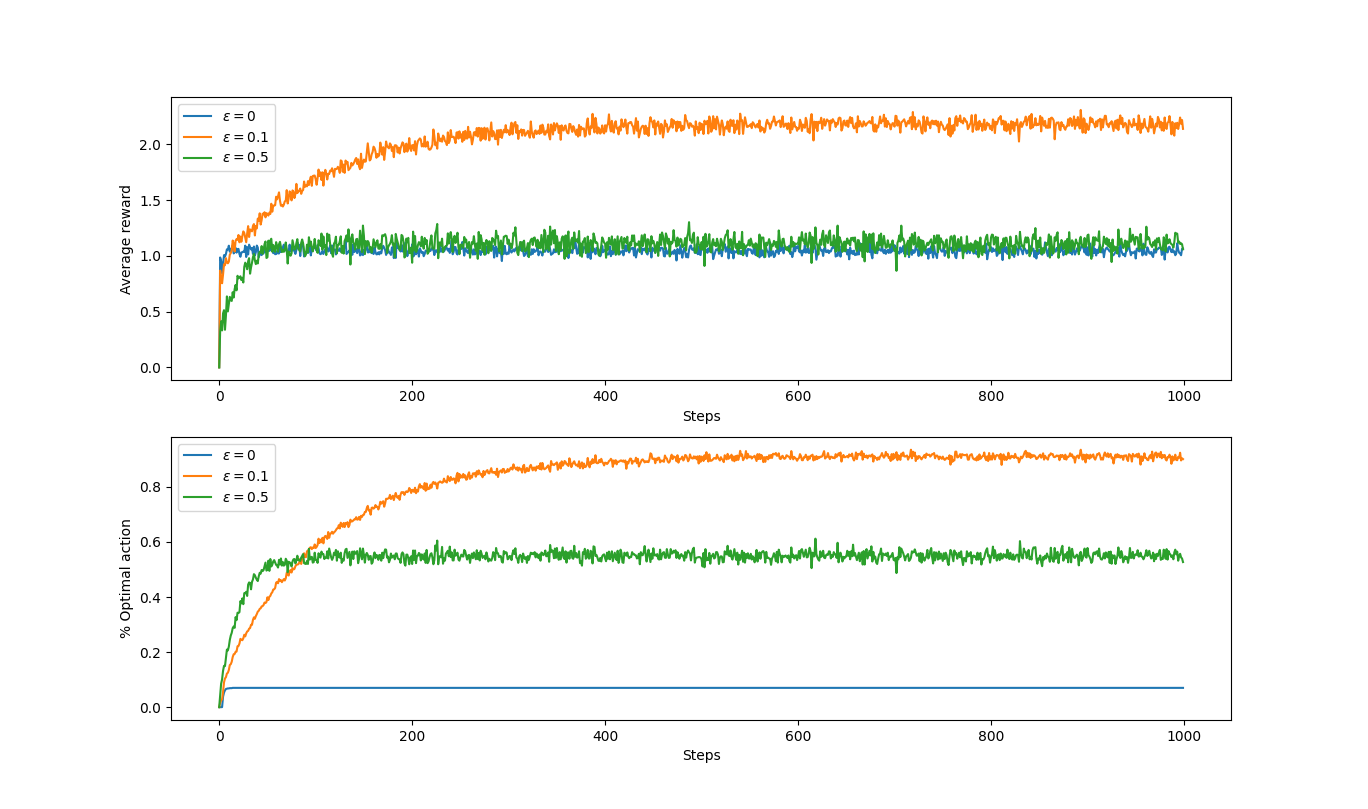
\includegraphics[width = 0.95 \textwidth]{1.4.1.png}    
\end{center}

\end{solution}

% --------------------------------------------------------------------------------

% -------------------------------------------------------------------------------- %

\begin{exercise}

Für welche Werte von $p \in \R$ gibt es ein signiertes Maß $\mu$ auf $(\N, 2^\N)$ mit $\mu(\Bbraces{x}) = x^p (-1)^x$?

\end{exercise}

% -------------------------------------------------------------------------------- %

\begin{solution}

\begin{align*}
    \mu:
        2^N \to \R,
        A \mapsto \sum_{x \in A} x^p (-1)^x
\end{align*}

Die Summe (Reihe) ist für $p < -1$ absolut konvergent, als Minorante der Geometrischen Reihe oder laut dem Leibniz-Kriterium, und $\mu$ damit wohldefiniert, und sonst divergent (nicht gegen $\infty$ oder $-\infty$).

\includegraphicsboxed{MassWHT1&2/MassWHT1&2 - Definition 6.1.png}

\begin{enumerate}

    \item $2^\N$ ist eine Sigmaalgebra.

    \item Der Wertebereich ist entweder $(-\infty, \infty]$ oder $[-\infty, \infty)$, weil
    
    \begin{align*}
        \Forall A \in 2^\N:
            \mu(A) \leq \mu(\N) < \infty.
    \end{align*}

    \item $\mu$ ist sigmaadditiv.
    
    \begin{align*}
        \Forall \vec A := (A_n) \subset 2^\N, ~\text{disjunkt}, A := \bigcup \vec A:
            \mu(A)
            =
            \sum_{x \in A}
                x^p (-1)^x
            =
            \sum_{n \in \N}
                \sum_{x \in A_n}
                    x^p (-1)^x
            \sum_{n \in \N}
                \mu(A_n)
    \end{align*}

\end{enumerate}

\end{solution}

% -------------------------------------------------------------------------------- %

% --------------------------------------------------------------------------------

\begin{exercise}

\phantom{}

\begin{enumerate}[label = (\alph*)]

  \item
  Definieren Sie Ring, Semiring, monotones System, Dynkin-System.
  
  \item
  Gegeben sei der Wahrscheinlichkeitsraum $(\Omega, \mathfrak{S}, \P)$. Für $A \in \mathfrak{S}$ sei
  
  \begin{align*}
    \mathfrak{U}(A) = \Bbraces{B: \P(A \cap B) = \P(A) \P(B)}
  \end{align*}
  
  das System aller Mengen, die von $A$ unabhängig sind. Zeigen Sie, dass $\mathfrak{U}(A)$ ein Dynkin-System ist.

\end{enumerate}

\end{exercise}

% --------------------------------------------------------------------------------

\begin{solution}

(a) Siehe Aufgabe 3 (a) \\

(b)

\begin{itemize}

  \item \Quote{Stabil bzgl. Differenzen von Teilmengen}: Seien $B, C \in \mathfrak{U}(A)$ mit $B \subseteq C$, dann gilt Folgendes.
  \begin{align*}
    \P(A \cap C \setminus B)
    & = \P(A) \P(C \setminus B)
    \Leftrightarrow \\
    \P(A) \P(B) + \P(A \cap C \setminus B)
    & = \P(A) \P(C \setminus B) + \P(A) \P(B)
      = \P(A) \P(C)
    \Leftrightarrow \\
    \P(A \cap C) + \P(A) \P(B)
      =\P(A \cap B) + \P(A) \P(B) + \P(A \cap C \setminus B)
    & = \P(A) \P(C) + \P(A \cap B)
  \end{align*}

  \item \Quote{Stabil bzgl. abzählbaren, disjunkten Vereinigungen}: Sei $(B_n) \in \mathfrak{D}$ disjunkt, dann
  \begin{align*}
    \P \pbraces{A \cap \sum_{n \in \N} B_n}
    =
    \sum_{n \in \N} \P(A \cap B_n)
    =
    \sum_{n \in \N} \P(A) \P(B_n)
    =
    \P(A) \P \pbraces{\sum_{n \in \N} B_n}.
  \end{align*}

  \item \Quote{Enthält Grundmenge}: $\P(A \cap \Omega) = \P(A) = \P(A) \P(\Omega)$

\end{itemize}

\end{solution}

% --------------------------------------------------------------------------------

% --------------------------------------------------------------------------------

\begin{exercise}[21]

Welche der folgenden Formeln sind Tautologien?

\begin{enumerate}[label = \alph*.]
    \item $(p_1 \to p_2) \to (p_3 \to p_4) \to ((p_1 \lor p_3) \to (p_2 \lor p_4))$. \\
    (Implikationen werden von rechts nach links geklammert;
    $A \to B \to C$ ist als Abkürzung für $(A \to (B \to C))$ zu lesen, NICHT als $((A \to B) \to C)$, und auch NICHT als $(A \to B) \land (B \to C)$.
    \item $(p_1 \to p_3) \to (p_2 \to p_3) \to ((p_1 \lor p_2) \to p_3)$.
    \item $(p_1 \to p_3) \to (p_2 \to p_3) \to ((p_1 \land p_2) \to p_3)$.
    \item $(p_1 \to p_2 \to p_3) \to ((p_1 \land p_2) \to p_3)$
    \item $(p_1 \to p_2) \lor (p_2 \to p_1)$.
\end{enumerate}

\end{exercise}

% --------------------------------------------------------------------------------

\begin{solution}

\phantom{}

\begin{enumerate}[label = \alph*.]

  \item
  
  \begin{align*}
    & (p_1 \to p_2) \to ((p_3 \to p_4) \to ((p_1 \lor p_3) \to (p_2 \lor p_4))) \\
    & \iff
    \neg (p_1 \to p_2) \lor ((p_3 \to p_4) \to ((p_1 \lor p_3) \to (p_2 \lor p_4))) \\
    & \iff
    (p_1 \land \neg p_2) \lor \neg (p_3 \to p_4) \lor ((p_1 \lor p_3) \to (p_2 \lor p_4)) \\
    & \iff
    (p_1 \land \neg p_2) \lor (p_3 \land \neg p_4) \lor \neg (p_1 \lor p_3) \lor p_2 \lor p_4 \\
    & \iff
    (p_1 \land \neg p_2) \lor (p_3 \land \neg p_4) \lor (\neg p_1 \land \neg p_3) \lor p_2 \lor p_4 \\
    & \stackrel{!}{\iff} \bot
  \end{align*}

  Dann sind aber alle Konjunktionen $\iff \bot$.
  Insbesondere, sind die letzten beiden $\iff \bot$, ihre Negationen also $\iff \top$.
  Weil aber die ersten beiden $\iff \bot$, müssen $p_1 \iff p_2 \iff \bot$, ihre Negationen aber $\iff \top$.
  Dann wäre die mittlere aber $\iff \top$.
  Widerspruch!

  \item

  \begin{align*}
    & (p_1 \to p_3) \to ((p_2 \to p_3) \to ((p_1 \lor p_2) \to p_3)) \\
    & \iff
    \neg (p_1 \to p_3) \lor ((p_2 \to p_3) \to ((p_1 \lor p_2) \to p_3)) \\
    & \iff
    (p_1 \land \neg p_3) \lor \neg (p_2 \to p_3) \lor ((p_1 \lor p_2) \to p_3) \\
    & \iff
    (p_1 \land \neg p_3) \lor (p_2 \land \neg p_3) \lor \neg (p_1 \lor p_2) \lor p_3 \\
    & \iff
    (p_1 \land \neg p_3) \lor (p_2 \land \neg p_3) \lor (\neg p_1 \land \neg p_2) \lor p3 \\
    & \stackrel{!}{\iff} \bot
  \end{align*}

  Dann sind aber alle Konjunktionen $\iff \bot$.
  Insbesondere, ist die letzte $\iff \bot$, ihre Negation also $\iff \top$.
  Die ersten beiden sind ebenfalls $\iff \bot$, also $p_1 \iff p_2 \iff \bot$, bzw. $\neg p_1 \iff \neg p_2 \iff \top$.
  Dann wäre aber die vorletzte $\iff \top$.
  Widerspruch!

  \item

  \begin{align*}
    & (p_1 \to p_3) \to ((p_2 \to p_3) \to ((p_1 \lor p_2) \to p_3)) \\
    & \stackrel{\text{b.}}{\iff}
    (p_1 \land \neg p_3) \lor (p_2 \land \neg p_3) \lor \neg p_1 \lor \neg p_2 \lor p_3 \\
    & \stackrel{!}{\iff} \bot
  \end{align*}

  Dann sind aber alle Konjunktionen $\iff \bot$.
  Insbesondere, sind die letzten drei $\iff \bot$, ihre Negationen also $\iff \top$.
  Dann wären aber auch die ersten beiden $\iff \top$.
  Widerspruch!

  \item

  \begin{align*}
    & (p_1 \to (p_2 \to p_3)) \to ((p_1 \land p_2) \to p_3) \\
    & \iff
    \neg (p_1 \to (p_2 \to p_3)) \lor ((p_1 \land p_2) \to p_3) \\
    & \iff
    (p_1 \land \neg (p_2 \to p_3)) \lor \neg (p_1 \land p_2) \lor p_3 \\
    & \iff
    (p_1 \land p_2 \land \neg p_3) \lor \neg p_1 \lor \neg p_2 \lor p_3 \\
    & \stackrel{!}{\iff} \bot
  \end{align*}

  Dann sind aber alle Disjunktionen $\iff \bot$.
  Insbesondere, sind die letzten drei $\iff \bot$, ihre Negationen also $\iff \top$.
  Dann wäre aber auch die erste $\iff \top$.
  Widerspruch!

  \item

  \begin{align*}
    & (p_1 \to p_2) \lor (p_2 \to p_1) \\
    & \iff
    \neg p_1 \lor p_2 \lor \neg p_2 \lor p_1 \\
    & \iff
    (p_1 \lor \neg p_1) \lor (p_2 \lor \neg p_2)
  \end{align*}

  Offensichtlich liegt eine Tautologie vor.

\end{enumerate}

\end{solution}

% --------------------------------------------------------------------------------

\begin{solution}

\phantom{}

\begin{enumerate}[label = \alph*.]

  \item Betrachte die Negation:

  \begin{align*}
    \neg ((p_1 \to p_2) \to (p_3 \to p_4) \to ((p_1 \lor p_3) \to (p_2 \lor p_4))) &\iff
    (p_1 \to p_2) \land \neg ((p_3 \to p_4) \to ((p_1 \lor p_3) \to (p_2 \lor p_4))) \\
    &\iff (p_1 \to p_2) \land (p_3 \to p_4) \land \neg ((p_1 \lor p_3) \to (p_2 \lor p_4)) \\
    &\iff (p_1 \to p_2) \land (p_3 \to p_4) \land (p_1 \lor p_3) \land \neg (p_2 \lor p_4) \\
    &\iff (\neg p_1 \lor p_2) \land (\neg p_3 \lor p_4) \land (p_1 \lor p_3) \land (\neg p_2 \land \neg p_4) \\
    &\iff (\neg p_2 \land \neg p_4) \land (\neg p_1 \lor p_2) \land (\neg p_3 \lor p_4) \land (p_1 \lor p_3)
  \end{align*}

  Aus der ersten und der zweiten Konjuktion erhalten wir $(\neg p_1 \land \neg p_2 \land \neg \neg p_4)$.
  Mit der dritten erhalten wir auch $(\neg p_4)$ und damit kann $(p_1 \lor p_3)$ nicht mehr erfüllt werden.
  Also ist die Negation der Aussage eine Kontradiktion und die originale Aussage eine Tautologie.

  \item Definiere $A := (p_1 \lor p_2) \to p_3, \quad B := p_2 \to p_3, \quad C:= p_1 \to p_3$. \\

  \begin{tabular}{|c|c|c|c|c|c|c|c|}
    \hline
    $p_1$ & $p_2$ & $p_3$ & $A$ & $B$ & $B \to A$
    & $C$ & $C \to B \to A$\\
    \hline
    $1$ & $1$ & $1$ & $1$ & $1$ & $1$ & $1$ & $1$\\
    \hline
    $1$ & $1$ & $0$ & $0$ & $0$ & $1$ & $0$ & $1$\\
    \hline
    $1$ & $0$ & $1$ & $1$ & $1$ & $1$ & $1$ & $1$\\
    \hline
    $1$ & $0$ & $0$ & $0$ & $1$ & $0$ & $0$ & $1$\\
    \hline
    $0$ & $1$ & $1$ & $1$ & $1$ & $1$ & $1$ & $1$\\
    \hline
    $0$ & $0$ & $1$ & $1$ & $1$ & $1$ & $1$ & $1$\\
    \hline
    $0$ & $1$ & $0$ & $0$ & $0$ & $1$ & $1$ & $1$\\
    \hline
    $0$ & $0$ & $0$ & $1$ & $1$ & $1$ & $1$ & $1$\\
    \hline
  \end{tabular} \\

  Es liegt also eine Tautologie vor.

  \item Definiere $A := (p_1 \land p_2) \to p_3, \quad B := p_2 \to p_3, \quad C:= p_1 \to p_3$. \\

  \begin{tabular}{|c|c|c|c|c|c|c|c|}
    \hline
    $p_1$ & $p_2$ & $p_3$ & $A$ & $B$ & $B \to A$
    & $C$ & $C \to B \to A$\\
    \hline
    $1$ & $1$ & $1$ & $1$ & $1$ & $1$ & $1$ & $1$\\
    \hline
    $1$ & $1$ & $0$ & $0$ & $0$ & $1$ & $0$ & $0$\\
    \hline
    $1$ & $0$ & $1$ & $1$ & $1$ & $1$ & $1$ & $1$\\
    \hline
    $1$ & $0$ & $0$ & $1$ & $1$ & $1$ & $0$ & $0$\\
    \hline
    $0$ & $1$ & $1$ & $1$ & $1$ & $1$ & $1$ & $1$\\
    \hline
    $0$ & $0$ & $1$ & $1$ & $1$ & $1$ & $1$ & $1$\\
    \hline
    $0$ & $1$ & $0$ & $1$ & $0$ & $0$ & $1$ & $1$\\
    \hline
    $0$ & $0$ & $0$ & $1$ & $1$ & $1$ & $1$ & $1$\\
    \hline
  \end{tabular} \\

  Es liegt also keine Tautologie vor.

  \item Definiere $A:= (p_1 \land p_2) \to p_3, \quad B := p_1 \to p_2 \to p_3$. \\

  \begin{tabular}{|c|c|c|c|c|c|}
    \hline
    $p_1$ & $p_2$ & $p_3$ & $A$ & $B$ & $B \to A$\\
    \hline
    $1$ & $1$ & $1$ & $1$ & $1$ & $1$\\
    \hline
    $1$ & $1$ & $0$ & $0$ & $0$ & $1$\\
    \hline
    $1$ & $0$ & $1$ & $1$ & $1$ & $1$\\
    \hline
    $1$ & $0$ & $0$ & $1$ & $1$ & $1$\\
    \hline
    $0$ & $1$ & $1$ & $1$ & $1$ & $1$\\
    \hline
    $0$ & $0$ & $1$ & $1$ & $1$ & $1$\\
    \hline
    $0$ & $1$ & $0$ & $1$ & $1$ & $1$\\
    \hline
    $0$ & $0$ & $0$ & $1$ & $1$ & $1$\\
    \hline
  \end{tabular} \\

  Es liegt also eine Tautologie vor.

  \item

  \begin{align*}
    (p_1 \to p_2) \lor (p_2 \to p_1) \iff (\neg p_1 \lor p_2) \lor (\neg p_2 \lor p_1) \iff (\neg p_1 \lor p_1) \lor (\neg p_2 \lor p_2).
  \end{align*}

  und es liegt eine Tautologie vor.

\end{enumerate}

\end{solution}

% --------------------------------------------------------------------------------


\phantom{}

Sei $b$ eine Belegung, $A$ eine Formel.
Statt $\hat{b}(A) = 1$ sagen wir auch \Quote{$b$ erfüllt die Formel $A$}.
In den nächsten 3 Aufgabe verstehen wir unter einer \Quote{Belegung} eine Funktion von der Menge $\Bbraces{p_1, \ldots, p_n}$ nach $\Bbraces{0, 1}$.

% --------------------------------------------------------------------------------

\begin{exercise}[22]

Sei $n \geq 2$.
Geben Sie eine Formel (in den Variablen $p_1, \ldots, p_n$) an, die von genau $n$ Belegungen erfüllt wird.

\end{exercise}

% --------------------------------------------------------------------------------

\begin{solution}

ToDo!

\end{solution}

% --------------------------------------------------------------------------------

% --------------------------------------------------------------------------------

\begin{exercise}[24]

Sei $n$ groß, $k \leq 2^n$.
Geben Sie eine Formel in den Variablen $p_1, \dots, p_n$ an, die von genau $k$ Belegungen erfüllt wird.
Versuchen Sie, eine möglichst kleine Formel zu finden (mit etwa $\Landau{n}$ Symbolen).

\end{exercise}

% --------------------------------------------------------------------------------

\begin{solution}

Wir stellen zuerst $k \in \{0,\dots,2^n-1\}$ binär dar:
\begin{align*}
  k = \sum_{i=0}^{n-1}a_i2^i, \quad a_i \in \{0,1\}.
\end{align*}
Als nächstes definieren wir für $i \in \{0,\dots,n-1\}$ disjunkte Mengen $B_i$
von Belegungen mit $|B_i| = 2^i$ wie folgt:
\begin{align*}
  B_{n-1} &:= \{b: b(p_1) = 0\} \\
  B_{n-2} &:= \{b: b(p_1) = 1, b(p_2) = 0\} \\
  &\vdots \\
  B_{1} &:= \{b: b(p_1) = 1, \dots, b(p_{n-2}) = 1, b(p_{n-1}) = 0\} \\
  B_{0} &:= \{b: b(p_1) = 1, \dots, b(p_{n-1}) = 1, b(p_{n}) = 0\}.
\end{align*}
Jetzt müssen wir noch Formeln $A_i$ finden, sodass die Menge aller Belegungen die $A_i$
erfüllen genau $B_i$ ist. Das funktioniert so:
\begin{align*}
  A_{n-1} &:= \neg p_1 \\
  A_{n-2} &:= p_1 \land \neg p_2 \\
  &\vdots \\
  A_{1} &:= p_1 \land \dots \land p_{n-2} \land \neg p_{n-1}\\
  A_{0} &:= p_1 \land \dots \land p_{n-1} \land \neg p_{n}\\
\end{align*}
Die Disjunktion aller $A_i$ liefert dann schließlich eine Formel, die von der
Vereinigung aller $B_i$ erfüllt wird.
Da die Mengen $B_i$ paarweise disjunkt sind, ist die Mächtigkeit von der Vereinigung
gleich der Summe der einzelnen Mächtigkeiten.

Für vorgegebenes $k$ betrachten wir also die Disjunktion aller $A_i$ mit $i \in \{i \in \{0,\dots,n-1\}: a_i \neq 0 \}$. \\
Wir verwenden also maximal $\sum_{i=0}^{n-1}2(n-i) + n - 1 = n^2 + 1 = O(n^2)$ Symbole. Es geht also anscheinend noch besser.

Zur Vollständigkeit halber sei noch gesagt, dass für $k = 2^n$ einfach die Formel $T$ gewählt werden kann.

Zusatz: Wir überlegen uns für $0 < l < m \leq n$ und die Formel $A_{n-l} \lor A_{n-m}$ die Äquivalenz
\begin{align*}
(p_1 \land p_2 \land \dots \land p_{l-1} \land \neg p_l) \lor (p_1 \land p_2 \land \dots \land p_{m-1} \land \neg p_m) \land \neg p_l) \lor (p_1 \land p_2 \land \dots \land p_{n-1} \land \neg p_n) \\
\Leftrightarrow (p_1 \land \dots \land p_{l-1}) \land (\neg p_l \lor (p_l \land \dots \land p_{m-1} \land \neg p_m) \lor (p_l \land \dots \land p_{n-1} \land \neg p_n)) \\
<<<<<<< HEAD
\Leftrightarrow (p_1 \land \dots \land p_{l-1}) \land (\neg p_l \lor ((p_l \land \dots \land p_{m-1}) \land (\neg p_m \lor (p_m \land \dots \land p_{n-1} \land \neg p_n)))) 
\end{align*}

\Leftrightarrow (p_1 \land \dots \land p_{l-1}) \land (\neg p_l \lor ((p_l \land \dots \land p_{m-1}) \land (\neg p_m \lor (p_m \land \dots \land p_{n-1} \land \neg p_n))))
\end{align*}
Zum Beispiel lässt sich für $k = 2^{n-1}$ folgende Vereinfachung vornehmen:
\begin{align*}
  A_{n-1} \lor \dots \lor A_{0} \iff \neg p_1 \lor (p_1 \land [\neg p_2 \lor (p_2 \land [\neg p_3 \lor (\dots [\neg p_{n-1} \land p_n)])])
\end{align*}
Damit können wir also die Anzahl der benötigten Symbole auf $O(n)$ reduzieren.

\end{solution}

% --------------------------------------------------------------------------------

\begin{solution}

Man kann auch eine leicht einzusehende Formel mit $\Landau{n \cdot 2^n}$ Symbolen konstruieren.
Dazu betrachten wir die Binärdarstellungen.

\begin{align*}
  \Forall k = 0, \ldots, 2^n - 1:
  \ExistsOnlyOne k_1, \ldots, k_n \in \Bbraces{0, 1}:
  k = \sum_{i=1}^n k_i 2^{i-1}
\end{align*}

In der folgenden Tabelle ist die Formel, die wir für allgemeine $k$ konstruieren werden, mal für die ersten paar $k$ aufgedröselt.
In der letzten Spalte steht jedes $W$ bzw. $F$, an der $k$-ten Stelle von links, für ein $p_k$ bzw. $\neg p_k$.
Diese werden horizontal mit $\land$ und anschließend vertikal mit $\lor$ verknüpft. \\

\begin{tabular}{|l|l|l|l|l|l|}
  \hline
  $k$ & $1$ & $2$ & $3$ & $4$ & $5$ \\
  \hline
  $k-1$ & $0$ & $1$ & $2$ & $3$ & $4$ \\
  \hline
  Binärdarschreibweise von $k-1$ & $0$ & $1$ & $10$ & $11$ & $100$ \\
  \hline
  Formel (angedeutet) & $W \cdots W$ & \makecell{$W W \cdots W$ \\ $F W \cdots W$} & \makecell{$W W W \cdots W$ \\ $F W W \cdots W$ \\ $W F W \cdots W$} & \makecell{$W W W \cdots W$ \\ $F W W \dots W$ \\ $W F W \dots W$ \\ $F F W \cdots W$} & \makecell{$W W W W \cdots W$ \\ $F W W W \dots W$ \\ $W F W W \dots W$ \\ $F F W W \cdots W$ \\ $W W F W \cdots W$} \\
  \hline
\end{tabular} \\

Um unsere Formel möglichst \Quote{schön} hinzuschreiben, definieren wir folgenden Ausdruck.

\begin{align*}
  (b \cdot \neg) p :=
  \begin{cases}
    p,      & b = 1 \\
    \neg p, & b = 0
  \end{cases},
  \quad
  b \in \Bbraces{0, 1}
\end{align*}

Die folgende Formel ist nun für genau $k = 0, \ldots, 2^n$ Belegungen von $p_1, \ldots, p_n$ wahr.
Man beachte, dass die leere Disjunktion ($k = 0$) stets falsch ist.

\begin{align*}
  \bigvee_{\ell = 0}^{k-1}
  \bigwedge_{i=1}^n
  (\ell_i \cdot \neg) p_i
\end{align*}

\end{solution}

% --------------------------------------------------------------------------------


\end{document}
